\begin{tikzpicture}
    \pgfplotsset{
        width=0.9\textwidth,
        height=0.3\textheight
    }
    \begin{axis}[
        % title={Temperature dependence of CuSO\(_4\cdot\)5H\(_2\)O solubility},
        xlabel={Measurements},
        ylabel={Measurements Required},
        xmin=0, xmax=3000,
        ymin=0, ymax=35000,
        xtick={0,500,1000,1500,2000,2500,3000},
        ytick={0, 5000,10000,15000,20000,25000,30000,35000},
        legend pos=north west,
        ymajorgrids=true,
        grid style=dashed,
    ]
    
    \addplot[
        color=blue,
        mark=square,
        ]
        coordinates {
        (200,4524)
        (400,4343)
        (600,8513)
        (800,23274)
        (1000,31855)
        (1200,26106)
        (1400,24753)
        (1600,23469)
        (1800,23865)
        (2000,20771)
        (2200,19028)
        (2400,18167)
        (2600,16882)
        (2800,15331)
        (3000,15137.0)
        };
        % \legend{CuSO\(_4\cdot\)5H\(_2\)O}
        
    \end{axis}
    \end{tikzpicture}